\chapter{【1级标题,三号黑体字】}
 
 [鼠标左键单击选择该段落,输入替换之。内容为小四号宋或楷体字。] 学位论文为了需要反映出作者确已掌握了坚实的基础理论和系统的专门知识,具有开阔的科学视野,对研究方案作了充分论证,因此,有关历史回顾和前人工作的综合评述,以及理论分析等,可以单独成章,用足够的文字叙述。正文是学位论文的核心部分,占主要篇幅,可以包括:调查对象、实验和观测方法、仪器设备、材料原料、实验和观测结果、计算方法和编程原理、数据资料、经过加工整理的图表、形成的论点和导出的结论等。\par
由于研究工作涉及的学科、选题、研究方法、工作进程、结果表达方式等有很大的差异,对正文内容不能作统一的规定。但是,必须实事求是,客观真切,准确完备,合乎逻辑,层次分明,简练可读。\par
\textcolor{red}{\textbf{图:}}\par
图包括曲线图、构造图、示意图、框图、流程图、记录图、地图、照片等。\par
图应具有“自明性”。\par
图应有编号。图的编号由“图”和从“1”开始的阿拉伯数字组成,图较多时,可分章编号。\par
图宜有图题,图题即图的名称,置于图的编号之后。图的编号和图题应置于图下方。\par
照片图要求主题和主要显示部分的轮廓鲜明,便于制版。如用放大缩小的复制品,必须清晰,反差适中。照片上应有表示目的物尺寸的标度。\par
图片示例1:
\begin{figure}[!htbp]
    \centering
    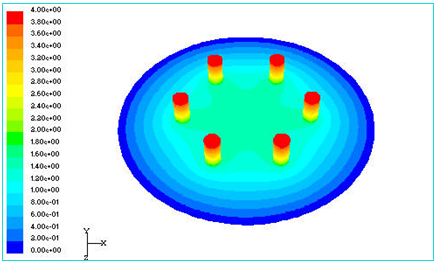
\includegraphics[width=0.5\textwidth]{figures/pic2-1.png}
    \caption{太合金多炭钢铁产品柱扭曲局部受力分析示意图}
    \label{fig:2-1}
\end{figure}

\textcolor{red}{\textbf{表:}}\par
表应具有“自明性”。\par
表应有编号。表的编号由“表”和从“1”开始的阿拉伯数字组成,表较多时,可分章编号。表较多时,可分章编号。\par
表宜有表题,表题即表的名称,置于表的编号之后。表的编号和表题应置于表上方。\par
表的编排,一般是内容和测试项目由左至右横读,数据依序竖读。\par
表的编排建议采用国际通行的三线表。\par
如某个表需要转页接排,在随后的各页上应重复表的编号。编号后跟表题(可省略)和“(续)”,置于表上方。\par
续表均应重复表头。\par
表格示例1:

\begin{table}[htbp]

    \centering
    \caption{国际单位制的基本单位}
    \label{tbl:2-1}
    \begin{tabularx}{0.8\textwidth}{*{3}{>{\centering\arraybackslash}X}}
        \toprule
        量的名称   & 单位名称     & 单位符号 \\ \midrule
        长度       & 米           & m        \\
        质量       & 千克(公斤)   & kg       \\
        时间       & 秒           & s        \\
        电流       & 安{[}培{]}   & A        \\
        热力学温度 & 开{[}尔文{]} & K        \\
        物质的量   & 摩{[}尔{]}   & mol      \\
        发光强度   & 坎{[}德拉{]} & cd       \\ \bottomrule
    \end{tabularx}
\end{table}

\textcolor{red}{\textbf{公式:}}\par
论文中的公式应另行起,并缩格书写,与周围文字留足够的空间区分开。\par
如有两个以上的公式,应用从“1”开始的阿拉伯数字进行编号,并将编号置于括号内。公式的编号右端对齐,公式与编号之间可用“…”连接。公式较多时,可分章编号。\par
公式示例1:
\begin{equation}
    \label{eqn:2}
    \phi=\frac{D_{p}^{2}}{150} \frac{\psi^{3}}{(1-\psi)^{2}}
\end{equation}
\begin{equation}
    \label{eqn:3}
    C_{2} =\frac{3.5}{D_{p}} \frac{(1-\psi)}{\psi^{3}}
\end{equation}

\noindent 式中  $\quad D_{p}$ —— 多孔质材料的平均粒子直径($m$);\par
$\psi$ —— 孔隙度(孔隙体积占总体积的百分比); \par
$\phi$ —— 特征渗透性或固有渗透性,与材料的结构性质有关($m^2$)。\par
较长的公式需要转行时,应尽可能在“=”处回行,或者在“+”、“-”“×”、“/”等记号处回行。\par
公式中分数线的横线,其长度应等于或略大于分子和分母中较长的一方。\par
如正文中书写分数,应尽量将其高度降低为一行。如将分数线书写为“/”,将根号改为负指数。\par
\newpage
公式示例2:\par
\begin{spacing}{2}
    \begin{math}
        \zihao{5} \quad\text{将}\;\dfrac{1}{\sqrt{2}}\;\text{写成}\; 1/\sqrt{2} \;\text{或}\; 2^{-1/2}。
    \end{math}
\end{spacing}

\textcolor{red}{\textbf{引文标注}}\par
论文中引用的文献的标注方法遵照GB/T 7714-2005,可采用顺序编码制,也可采用著者-出版年制,但全文必须统一。\par
\textcolor{red}{\textbf{注释}}\par
当论文中的字、词或短语,需要进一步加以说明,而又没有具体的文献来源时,用注释。注释一般在社会科学中用得较多。\par
应控制论文中的注释数量,不宜过多。\par
由于论文篇幅较长,建议采用文中编号加“脚注”的方式。最好不用采用文中编号加“尾注”。\par

\section{【2级标题,小三号黑体字】 }
 [鼠标左键单击选择该段落,输入替换之。内容为小四号宋或楷体字。]
\subsection{【3级标题,四号黑体字】 }
[鼠标左键单击选择该段落,输入替换之。内容为小四号宋或楷体字。]